\documentclass[oneside]{book}
\usepackage[margin=1.0in]{geometry}
\usepackage{authblk}
\usepackage{graphicx}
\usepackage{float}
\usepackage{hyperref}

\usepackage[binary-units=true]{siunitx}

\usepackage[utf8]{inputenc} % Define the input encoding
\usepackage[T1]{fontenc}
\usepackage[USenglish]{babel} % Define language used
\usepackage{amsmath,amsfonts,amssymb}
\usepackage{amsthm} % Gives us plain, definition, and remark to use in \theoremstyle{style}
\usepackage{mathtools} % Allow for text and math in align* environment.
\usepackage{thmtools}

\usepackage[
backend=biber,
style=numeric]{biblatex} % Must include citation somewhere in document to print bibliography
\renewcommand{\subtitlepunct}{\addcolon\addspace}

\usepackage{hyperref} % Generate hyperlinks to referenced items
\usepackage[noabbrev,nameinlink]{cleveref} % Fancy cross-references in the document everywhere
\usepackage{nameref} % Can make references by name to places
\usepackage{caption} % Allows for greater control over captions in figure, algorithm, table, etc. environments
\usepackage{subcaption} % Allows for multiple figures in one Figure environment
\usepackage[binary-units=true]{siunitx} % Gives us ways to typeset units for stuff
\usepackage{csquotes} % Context-sensitive quotation facilities
\usepackage{chngcntr} % Allows us to tamper with the counter a little more
\usepackage{empheq} % Allow boxing of equations in special math environments
\usepackage{xcolor} % Gives access to coloring text in environments or just text, MUST be before tikz
\usepackage{nth} % Programmatically give ordinal numbers in the text

% Programmatically give dates in documents.
\usepackage[useregional]{datetime2}
% \selectlanguage{english}

% Color hyperlinks differently
\hypersetup{
  colorlinks=true,
  linkcolor=blue,
  filecolor=magenta,
  urlcolor=cyan,
  citecolor=red,
}

% These packages require the use of the -shell-escape flag when compiling
\usepackage{minted}
\crefname{lstlisting}{listing}{listings}
\Crefname{lstlisting}{Listing}{Listings}
\def\mintedbashargs{
  frame=lines, % Surround the source code with lines on top and bottom
  linenos, % We want to show line numbers for each line in the margin
  % Colors used here are xcolor X11 colors.
  % style=fruity, % Use the fruity color scheme. Best for use on black backgrounds. Use for code blocks.
  % bgcolor=black, % Set the background used
  % style=emacs,
  % bgcolor=white,
  autogobble=true, % Automatically remove shared indentation from files
  breaklines=true, % Break lines that are too long at convenient locations
}
\newcommand{\makenewmintedfiles}[1]{
  \newminted[bashsource]{bash}{#1} % Use with \begin{bashsource} code \end{bashsource}

  \newmintedfile[bashsourcefile]{bash}{#1} % Use with \bashsourcefile[additional-options]{Filename}
}
\expandafter\makenewmintedfiles\expandafter{\mintedbashargs}
\newmintinline[bashinline]{bash}{% Use with \bashinline{code}
  style=emacs,
  bgcolor=white,
}

% Extra commands we choose to define
\newcommand{\file}[1]{\texttt{#1}}

% Add bibliography files here
\addbibresource{../References.bib}

% Add paths to search for images here
\graphicspath{{./Images/}}

% Enable the printing of a glossary
\usepackage[toc,acronym,writeglslabels]{glossaries}
\makeglossaries{}
\begin{titlepage}
  \title{Chipyard SoC Design Framework}
  \author{Alexander Lukens \and Karl Hallsby}
  \date{Last Edited: \today}
  \affil{Illinois Institute of Technology}
\end{titlepage}

\begin{document}
\nocite{chipyard}

\frontmatter
\maketitle
\tableofcontents

\mainmatter{}
\chapter{Setup}\label{chap:Setup}
\section{Introduction}\label{sec:Introduction}
This document is intended to serve as a record of the work performed for the ECE 497 special project supervised by Professor Jia Wang during the Spring 2021 semester.
In this document, we will specify how our project repository was created, outline issues we ran into, and provide guidance on how to better setup the Chipyard Framework.

Chipyard is a framework for designing, \glslink{elaboration}{elaborating}, simulating, testing, and building \Gls{riscv} CPU designs.
It provides the functionality to define a set of standard CPU designs, but also allows for the end-user to describe their own custom designs and integrate them as first-class citizens in the framework.
It also provides a toolkit for verifying that \glslink{elaboration}{elaborated} CPU designs meet the \Gls{riscv} \Gls{isa} standard, ensuring designed chips are compliant.
There are also tools for writing the \glslink{elaboration}{elaborated} designs out to \gls{fpga} bitstreams, so that simulation can be sped up and execution can occur on \glspl{softcore}.
Lastly, Chipyard includes tools for a VLSI-design workflow, to implement the \glslink{elaboration}{elaborated} CPU design on actual silicon.

\section{Project Environment}\label{sec:Project_Environment}
The first step to using the Chipyard Framework is creating a project environment and obtaining all of the Chipyard dependencies.
In this document, we assume you are using Ubuntu 20.04 LTS, running in a virtual machine with \textbf{at least}:
\begin{itemize}
\item 4 cores
\item \SI{16}{\giga\byte} of RAM, or more
\item \SI{250}{\giga\byte} disk image
\end{itemize}

Much of the disk space that has been allocated will be utilized, as the entire RISC-V toolchain and Xilinx Vivado Suite require a large amount of disk space.

This document will work equally well in other distributions (Fedora, CentOS, OpenSuSE, Archlinux, etc.), so long as the versions of the dependencies are matched.
Chipyard has explicit support for CentOS, extending to Fedora and RHEL as well.

Using Linux as the native operating system, rather than as a virtual machine is the preferred way of working with Chipyard.
This gives the running system \emph{all} available system resources and removes the virtual machine execution penalty.

\section{Document Typesetting}\label{sec:Doc_Typesetting}
This document makes use of a variety of different fonts and colors to denote different aspects of this work.
Each of the different font settings are explained here.

\begin{description}
\item[\texttt{Teletype Text}] Computing-related topics/items.
  This is typically used to denote terms you will see in this document, repository, and other materials surroudning this topic, but do not correlate to any of the other options here.
\item[\file{file/path}] A relative file path.
  This is typically used with \file{chipyard/subdir}, meaning you should move to the specified subdirectory or file \emph{inside} of the Chipyard subdirectory.
  They will only look this way when a file is specified by itself, not in any commands.
\item[\file{/file/path}] An absolute file path.
  When specified this way, you must provide the entire path specified.
  They will only look this way when a file is specified by itself, not in any commands.
% NOTE: The textcolors below should match the ones defined in hypersetup in doc.tex!
\item[\textnormal{\textcolor{blue}{Blue Text}}] A link within this document.
  Clicking other word(s) that look like this will take you to a different place inside this document.
\item[\textnormal{\textcolor{cyan}{URL Link}}] A link to take you outside of this document.
\item[\bashinline{cmd-to-run}] A command to run in your terminal.
  We assume you are using the Bash shell.
\end{description}

In addition, we make use of \gls{man} syntax here.
This means that text inside of angle brackes is mandatory, inside of square brackets is optional, and the vertical pipe is an ``or.''
An example is shown in \Cref{lst:man_Syntax}.

\begin{listing}[h!tbp]
\begin{bashsource}
command <mandatory-arg> [optional-arg-1] [optional-arg-2a | optional-arg-2b]
\end{bashsource}
\caption{\gls{man} Syntax}
\label{lst:man_Syntax}
\end{listing}

\begin{blackbox}
  Text inside black boxes, like this one, is meant to provide an area for notes that should be remembered.
  For example, some of these provide reminders to \glslink{multithread}{parallelize} code compilation to speed up the process.
\end{blackbox}

\section{Building Chipyard}\label{sec:Building_Chipyard}
Here, we present the necessary steps to retrieving all the dependencies required to set up Chipyard for local development and simulation use.
The larger code listings shown in this document is gathered in the \file{code} subdirectory of this document's project directory.
We developed this documentation using version \href{https://github.com/ucb-bar/chipyard/releases/tag/1.4.0}{\textbf{1.4.0}}\footnote{Git Commit Hash: \href{https://github.com/ucb-bar/chipyard/commit/58076cfb260a3be502d6d1c25b577da39277a7fc}{58076cfb260a3be502d6d1c25b577da39277a7fc}} of Chipyard.

\subsection{Chipyard Dependencies}\label{sec:Chipyard_Dependencies}
To gather the Chipyard dependencies, follow the \href{https://chipyard.readthedocs.io/en/latest/}{Chipyard} documentation closely.
Specifically, the \href{https://chipyard.readthedocs.io/en/latest/Chipyard-Basics/Initial-Repo-Setup.html}{Section 1.4} of the documentation outlines how to prepare your operating system for development using the Chipyard framework.

A paraphrased reproduction of these steps are shown below.

\subsubsection{Retrieve/Install Dependencies}\label{sec:Retrive_Install_Dependencies}
Chipyard relies on numerous dependencies and libraries to read files and build the required Verilog files.
In addition, Chipyard relies on \gls{sbt}, because a majority of Chipyard and its dependencies are written in Scala.

\Cref{lst:Ubuntu_Chipyard_Deps_Setup} is a script that handles fetching and installing all the dependencies for you.
Note that this does \textbf{not} work for installing the dependencies for Linux distributions that do not use the \texttt{apt} package manager.

\begin{listing}[h!tbp]
\bashsourcefile{./code/ubuntu-chipyard-deps-setup.sh}
\caption{Fetch Chipyard Dependencies using \texttt{apt} on Ubuntu}
\label{lst:Ubuntu_Chipyard_Deps_Setup}
\end{listing}

\subsubsection{Build Verilator from Source}\label{sec:Build_Verilator_from_Source}
Chipyard's documentation recommends building \href{https://www.veripool.org/wiki/verilator}{Verilator} (an open-source (System)Verilog simulator and compiler) from \gls{source}.

A small script has been provided that handles this for you in \Cref{lst:Build_Verilator_from_Source}.
Note that this does \textbf{not} work for installing the dependencies required to build Verilator for Linux distributions that do not use the \texttt{apt} package manager.

\begin{listing}[h!tbp]
\bashsourcefile{./code/build-verilator.sh}
\caption{Building Verilator from \Gls{source} on Debian-derivative Linux Distributions}
\label{lst:Build_Verilator_from_Source}
\end{listing}

\subsubsection{Fetching Chipyard and its Direct Dependencies}\label{sec:Fetching_Chipyard_Direct_Dependencies}
In addition to the library and external programs that Chipyard depends on, it also uses git submodules to track direct dependencies.
Direct dependencies are projects that Chipyard directly relies on.
These include SiFive's CPU designs, the \nameref{sec:BOOM_Generator} CPU design, \nameref{sec:Rocket_Chip}, and several others.

\Cref{lst:Fetch_Chipyard_and_Submodules} has been provided that handles this for you.

\begin{listing}[h!tbp]
\bashsourcefile{./code/fetch-chipyard-and-submodules.sh}
\caption{Fetch Chipyard and Submodules}
\label{lst:Fetch_Chipyard_and_Submodules}
\end{listing}

\subsection{Building a Toolchain}\label{sec:Building_Toolchain}
To compile programs from C to RISC-V instructions, there are several tools you need, when grouped together is called a toolchain.
Your cloned Chipyard repository contains a script to install these.
You can run the script to build a good general-purpose toolchain using \Cref{lst:Build_RISCV_Toolchain} or \Cref{lst:Build_RISCV_Toolchain-Parallel} while inside your local copy of the cloned Chipyard repository.

\begin{listing}[h!tbp]
\begin{bashsource}
./scripts/build-toolchains.sh riscv-tools
\end{bashsource}
\caption{Build \Gls{riscv} Toolchain}
\label{lst:Build_RISCV_Toolchain}
\end{listing}

\begin{listing}[h!tbp]
\begin{bashsource}
export MAKEFLAGS=-j[N]; ./scripts/build-toolchains.sh riscv-tools}
\end{bashsource}
\caption{Parallel Build \Gls{riscv} Toolchain}
\label{lst:Build_RISCV_Toolchain-Parallel}
\end{listing}

\subsubsection{Environment Variables}\label{sec:Environment_Variables}
Once the toolchain is built, an environment-setup script is emitted to the root of your local copy of Chipyard, with the name \file{env.sh} (located at \file{chipyard/env.sh}).
This file is a bash script that changes your \texttt{PATH}, \texttt{RISCV}, and \texttt{LD\_LIBRARY\_PATH} environment variables so that Chipyard can find everything it needs.

To alleviate any issues that may occur due to misconfigured or non-existent environment variables, we recommend you do one of the following:
\begin{enumerate}
\item Add the line \bashinline{source /path/to/chipyard/env.sh} to the end of your \file{.bashrc} file in your home directory.
  After adding this to your \file{.bashrc} file, restart your shell, or re-\bashinline{source} your \file{.bashrc} and continue.
\item Install the \href{https://direnv.net/}{\texttt{direnv}} package and use it to automatically change your environment variables for you, instead of having them constantly loaded the way the previous option does.
\end{enumerate}

\section{Example CPU Design}\label{sec:Example_CPU_Design}
In this section, we show how to build and simulate the default CPU Chipyard defines.
This particular CPU is relatively easy to \glslink{elaboration}{elaborate}, requiring just \SI{6}{\giga\byte} of memory.

\subsection{Building the Example Design}\label{sec:Building_Example_Design}
To build the example design that Chipyard defines, all you must do is enter one of the simulator directories and type \bashinline{make}.
This \textbf{does} require that both the RISC-V toolchain you built and Verilator Verilog simulator be loaded into your environment~(see \Cref{sec:Environment_Variables}).
If one of these is not available, the \texttt{make} command will print out an error message why it is failing.

\begin{blackbox}
  We strongly recommended that you parallelize the \gls{elaboration} of the CPU design.
  You can achieve this by passing the \texttt{-j [N]} flag to \texttt{make}.
  You may replace the \texttt{[N]} with a number to indicate the number of your CPU cores to use for building.

  \textbf{If you omit the \texttt{[N]} entirely, the build system will use ALL cores!}

  The \gls{elaboration} of the default \texttt{RocketConfig} requires about \SI{6.5}{\giga\byte} of main memory.
  Otherwise the process will fail with \bashinline{make: *** [firrtl_temp] Error 137} which is most likely related to limited resources.
  Other configurations might require even more main memory~\cite{chipyard}.

  Using many cores increases the amount of system memory required, so be sure that you do not request too many cores be used if you are limited on memory.
\end{blackbox}

The commands to run, in order, are:
\begin{enumerate}
\item \bashinline{cd chipyard/sims/verilator}
\item \bashinline{make}
\end{enumerate}

\begin{blackbox}
  To parallelize the Verilator simulator, you must pass the \texttt{VERILATOR\_THREADS} variable to the \texttt{make} command.
  \textbf{You must \glslink{multithread}{parallelize} Verilator during building, not just during simulation time.}
  As an example, \bashinline{make VERILATOR_THREADS=4} will inform Verilator to use 4 cores/threads when simulating the design.
\end{blackbox}

Finishing the \gls{elaboration} of the design produces an \textbf{executable} called \file{simulator-chipyard-RocketConfig}.
This executable is capable of running any RISC-V compatible code.

\subsection{Running the Example Design}\label{sec:Running_Example_Design}
To run arbitrary code, the executable takes the ELF file of the program to run as a parameter.
An example of the command to run is shown in \Cref{lst:Running_Example_Design}.

\begin{listing}[h!tbp]
\begin{bashsource}
./simulator-chipyard-RocketConfig $RISCV/riscv64-unknown-elf/share/riscv-tests/isa/rv64ui-p-simple
\end{bashsource}
\caption{Run Arbitrary RISC-V Programs using Example Design}
\label{lst:Running_Example_Design}
\end{listing}

Chipyard also provides a quality-of-life \texttt{make} directive when running these programs, shown in \Cref{lst:Running_Example_Design-Make}.

\begin{listing}[h!tbp]
\begin{bashsource}
make run-binary BINARY=<path/to/riscv/elf>
\end{bashsource}
\caption{\texttt{make} command to run arbitrary RISC-V programs using Example Design}
\label{lst:Running_Example_Design-Make}
\end{listing}

Using the \texttt{make} directive also allows the built design to accept many common command line options, including redirecting \texttt{STDOUT} to a file.

\subsection{Simulating the Example Design}\label{sec:Simulating_Example_Design}
Similar to \Cref{sec:Running_Example_Design}, the simulations are actually just a set of \Gls{riscv} programs designed to test the built designs.
There are two main commands for running the simulation test suite: \Cref{lst:ASM_Tests,lst:Run_Benchmark_Tests}.

\begin{listing}[h!tbp]
\begin{bashsource}
make run-asm-tests
\end{bashsource}
\caption{Run Compliance Tests to RISC-V ISA}
\label{lst:ASM_Tests}
\end{listing}

\begin{listing}[h!tbp]
\begin{bashsource}
make run-bmark-tests
\end{bashsource}
\caption{Run Benchmark Tests}
\label{lst:Run_Benchmark_Tests}
\end{listing}

\section{Xilinx Vivado Suite Installation}\label{sec:Xilinx_Vivado_Suide_Install}
It is important to install the \href{https://www.xilinx.com/support/download.html}{Xilinx Vivado Suite} if any work regarding an \Gls{fpga} is to be conducted.
The suite features tools a variety of tools used in teh design, building, and testing of hardware designs using \glspl{softcore}.

Vivado, one of the programs in the suite, is used for all aspects of managing \Glspl{fpga}.
It handles the setup process for the \Gls{fpga}, writing the bitstream to the \Gls{fpga}, among many other features.

We used the ``offline installation'' version of the Xilinx Unified Installer (version 2020.2), so no \nth{3} party libraries would need to be installed.
Xilinx is supported for a variety of operating systems, including Ubuntu\footnote{Xilinx only officially offers support for Ubuntu 16.04.2 LTS, but it should work on any Ubuntu version since then.}

When conducting the installation, be sure to select the ``Vitis'' installation target instead of just selecting ``Vivado''.
Installing Vitis will install both Vivado, and all other Xilinx tools needed for implementing FPGA projects.

\section{Other Useful Projects}\label{sec:Other_Useful_Projects}
\subsection{Freedom E SDK}\label{sec:Freedom_E_SDK}
\href{https://github.com/sifive/freedom-e-sdk}{This repository} is maintained by SiFive, and provides several useful tools for designing, uploading, and debugging software to FPGA devices~\cite{freedomESDK}.
This repository is specifically meant for use with SiFive IP, but can still be utilized for Chipyard projects with some modification.

For setting up this repository with its dependencies and compiling the necessary programs, refer to their \href{https://github.com/sifive/freedom-e-sdk#setting-up-the-sdk}{Prerequisites section}.

\subsection{Freedom Tools}\label{sec:Freedom_Tools}
\href{https://github.com/sifive/freedom-tools}{This repository} is maintained by SiFive~\cite{freedomTools}.
It will be used to generate several tools that will be used during this project, such as:
\begin{itemize}
\item The GCC cross-compiler for RISC-V (and many extension sets of RISC-V)
\item OpenOCD, which assists users in debugging their FPGA designs
\item RISC-V QEMU for system testing through emulation
\item And other useful software.
\end{itemize}
% TODO: Explain what each of these programs does.

These tools take a considerable amount of time and disk space to compile so it is best to run the \texttt{make} command as \mintinline{bash}{make -j`nproc`} to parallelize compiling.
Note that this will consume many system resources, and you should be prepared to have an unresponsive machine while the system is building these tools.

%%% Local Variables:
%%% mode: latex
%%% TeX-master: "../doc"
%%% End:


\chapter{Repository Deep Dive}\label{chap:Repository_Deep_Dive}
In this section, we lightly discuss each of the subdirectories present within the root of Chipyard, take note of any particularly important files, and demonstrate how this entire system is put together.

\section{Makefiles, or the Glue of this Framework}\label{sec:Makefiles_in_Chipyard}
Chipyard makes \textbf{heavy} use of Makefiles to pull together and automate various parts of the build system.
Variables and/or values that are shared between different ways of building systems are higher in the directory structure.

Thus, some of the most overarching commands and variables for this project are defined in \file{chipyard/variables.mk}.
One of the first things defined within this file are numerous output messages.

\subsection{\texttt{SUB\_PROJECT}}\label{subsec:Makefile_SUB_PROJECT}
The first notable part of the \file{variables.mk} file is the \texttt{SUB\_PROJECT} defaulting variable.
This particular variable is what allows for easy re-configuration of the entire framework to support elaborating your own CPU designs.
By changing this file between one of the well-defined options, one can easily re-use major portions of Chipyard's architecture.

For example, to switch from a CPU defined by Chipyard to one that is uses the Hwacha accelerator, one just needs to say \mintinline{bash}{make SUB_PROJCT=hwacha}, and all the necessary configuration variables are changed.

\subsection{Building Each Subproject}\label{subsec:Building_Each_Subproject}
The next notable part of this file is its large \mintinline{make}{ifeq ... endif} blocks.
Each one of these defines a different subproject that can be built and elaborated upon by Chipyard and its surrounding framework.
These subproject defining blocks each define multiple higher-level variables which are the variables that are actually used to build and test each of the CPUs.
Each of the variables is important, and Chipyard provided documentation for each variable inside \file{variables.mk}.
However, additional information that we gathered through trial-and-error is presented below.

\begin{description}
\item[\texttt{SUB\_PROJECT}] This corresponds to one of the projects in the \file{chipyard/generators} directory.
  More formally, it is defined by one of the entries in the \file{build.sbt} files in the respective generators directory, and by the main \file{build.sbt} file in the root of Chipyard.
\item[\texttt{SBT\_PROJECT}] This corresponds to a top-level of the repository of the chip to build.
  This is where many of the higher-level constructs, such as the test harness and test bench are defined from.
\item[\texttt{MODEL}] The model is the top-level module of the project that should be used by Chisel.
  Normally, this should be defined to the be same as the test harness, but does not necessarily have to be.
\item[\texttt{VLOG\_MODEL}] This is the top-level module of the project that should be used by FIRRTL/Verilog.
  Like \texttt{MODEL}, this is usually the same as the test harness, but does not necessarily need to be.
\item[\texttt{MODEL\_PACKAGE}] This is the Scala package that is used to find the overall model of the CPU.\@
  This should correspond to the \mintinline{scala}{package <packageName>} in a Scala CPU configuration file.
\item[\texttt{CONFIG}] This defines the parameters that should be used for the project.
  Typically, this is used to select one of the CPU configurations defined in the \texttt{SBT\_PROJECT}.
\item[\texttt{CONFIG\_PACKAGE}] This is the Scala package that defines the \texttt{Config} class.
  This file \textbf{MUST} contain the class definition for \texttt{Config}, meaning \mintinline{scala}{object Config} must be present.
\item[\texttt{GENERATOR\_PACKAGE}] This is the Scala package that defines the \texttt{Generator} class.
  This file \textbf{MUST} contain the class definition for \texttt{Generator}, meaning \mintinline{scala}{object Generator} must be present.
\item[\texttt{TB}] This defines the test bench wrapper that extends over the test harness to allow for simulation in a Verilog simulator.
\item[\texttt{TOP}] This is the top-level module of the project.
  Typically, this is the module instantiated by the test harness.
\end{description}

\section{\file{build.sbt}}\label{sec:build.sbt}
There are two main \file{build.sbt} files that you should be aware of.
There is a \file{build.sbt} for each of the generator subdirectories.
These define some metadata information about each of the projects, such as the name of the design, the authors of the design, the targeted \texttt{sbt} version, and others.

However, the \file{build.sbt} file in the root of Chipyard is a metadata file not just for Chipyard itself, but also pulls together all the dependencies in \file{chipyard/generators/} so that they all can be elaborated upon with Chipyard.

% TODO: Rework this paragraph about circular dependency in main build.sbt file.
This file is also the one that should be used for defining your \emph{own} CPU.\@
Note that this means you are building your own Verilog code which defines the generation rules for a CPU.\@
However, one must be careful that they do not introduce circular dependencies into the dependency graph between the CPU generation and elaboration tools.
Even though Scala has support for lazy evaluation, it does not completely extend to dependency evaluation, and the entire system can fall apart.
This does \emph{not} mean that you use this to build a new CPU on top of the architecture already defined by Chipyard, or any other CPU.\@
However, you can use other CPU-generating systems inside your design.

\subsection{About}\label{sec:About_Verilator_Simulator}
The primary way to simulate SoCs' designed using the Chipyard framework is via Verilator simulations.
The directory for verilator is \file{chipyard/sims/verilator}.
An example simulation can be run by using \mintinline{bash}{make} in the verilator directory.
Running the \texttt{make} command produces a simulator executable in the verilator directory.

Custom Chipyard configs can be simulated by running \mintinline{bash}{make CONFIG=<your custom config>}.
For example, if your project name was ``TestConfig'', running \mintinline{bash}{make CONFIG=TestConfig} would create an executable called \file{simulator-chipyard-TestConfig} in the \file{verilator} directory.
Custom RISCV code can be run by using the command \mintinline{bash}{./simulator-chipyard-TestConfig /path/to/riscv/executable} from the \file{chipyard/sims/verilator} directory.

\section{Generators}\label{sec:Generators}
In this section, we look at each of the subdirectories inside the \file{chipyard/generators} subdirectory in turn.
Each of the CPU generators presented below are each slightly unique in their implementation of the open RISC-V ISA.\@

\subsection{BOOM}\label{sec:BOOM_Generator}
\nocite{boomHomepage}
\nocite{boomPaper}
BOOM~(Berkeley Out-of-Order Machine) is a CPU defined and built by Univerity of California at Berkeley that implements the RISC-V Instruction Set Architecture (ISA).
Its claim to fame is that it can execute RISC-V instructions out-of-order, thereby drastically improving performance.
It is designed to be highly performant, synthesizable, and parameterizable.

BOOM includes support for the following operations:
\begin{itemize}
\item Floating Point (IEEE 754--2008)
\item Atomic Operations
\item Caching
\item Virtual Memory
\end{itemize}
In addition, BOOM supports external debugging.
Microarchitectural documentation can be found \href{https://docs.boom-core.org/en/latest/}{here}.
The GitHub organization and its development can be found \href{https://github.com/riscv-boom}{here}.

These CPU definitions are used by \nameref{sec:Chipyard_Generator} when elaborating CPU designs defined by the end-programmer.

\subsection{Chipyard}\label{sec:Chipyard_Generator}
This is the main source of truth inside this repository.
Here is where all of the code required to get these disparate CPUs to work and build together is located.
Typically, very little editing is needed to be done here.
Most of the editing in this repository comes in the form of defining your own CPUs, which are themselves defined in terms of other CPUs or other lower-level Chipyard constructs.

\subsection{cva6}\label{sec:cva6_Generator}
\nocite{cva6Github}
\nocite{zaruba2019cost}
cva6 is a 6-stage, single issue, in-order CPU.\@
This means that unlike the \nameref{sec:BOOM_Generator} design, instructions are \emph{always} executed in order.
It fully implements the 64-bit RISC-V instruction set, and several extensions, including:
\begin{description}
\item[I] Base Integer (the base 64-bit instruction set)
\item[M] Integer Multiplication and Division
\item[A] Atomic Operations
\item[C] Compression/Decompression Operations
\end{description}
In addition, it supports three different privilege levels, M, S, and U.
This allows the chip to run a full Unix-like operating system.

\subsection{Gemmini}\label{sec:Gemmini_Generator}
\nocite{gemminiGithub}
\nocite{gemminiPaper}
Gemmini is not a CPU, per se.
Instead, it is a CPU \emph{accelerator}, implemented alongside another CPU, such as a \nameref{sec:BOOM_Generator} or \nameref{sec:Rocket_Chip} design.
It is intended for hardware-level matrix operations, such as matrix multiplication, machine learning, and other SIMD\footnote{Single Instruction Multiple Data} operations.
A general logic design for the Gemmini accelerators is shown in \Cref{fig:Gemmini_Accelerator}.

\begin{figure}[h!tbp]
  \centering
  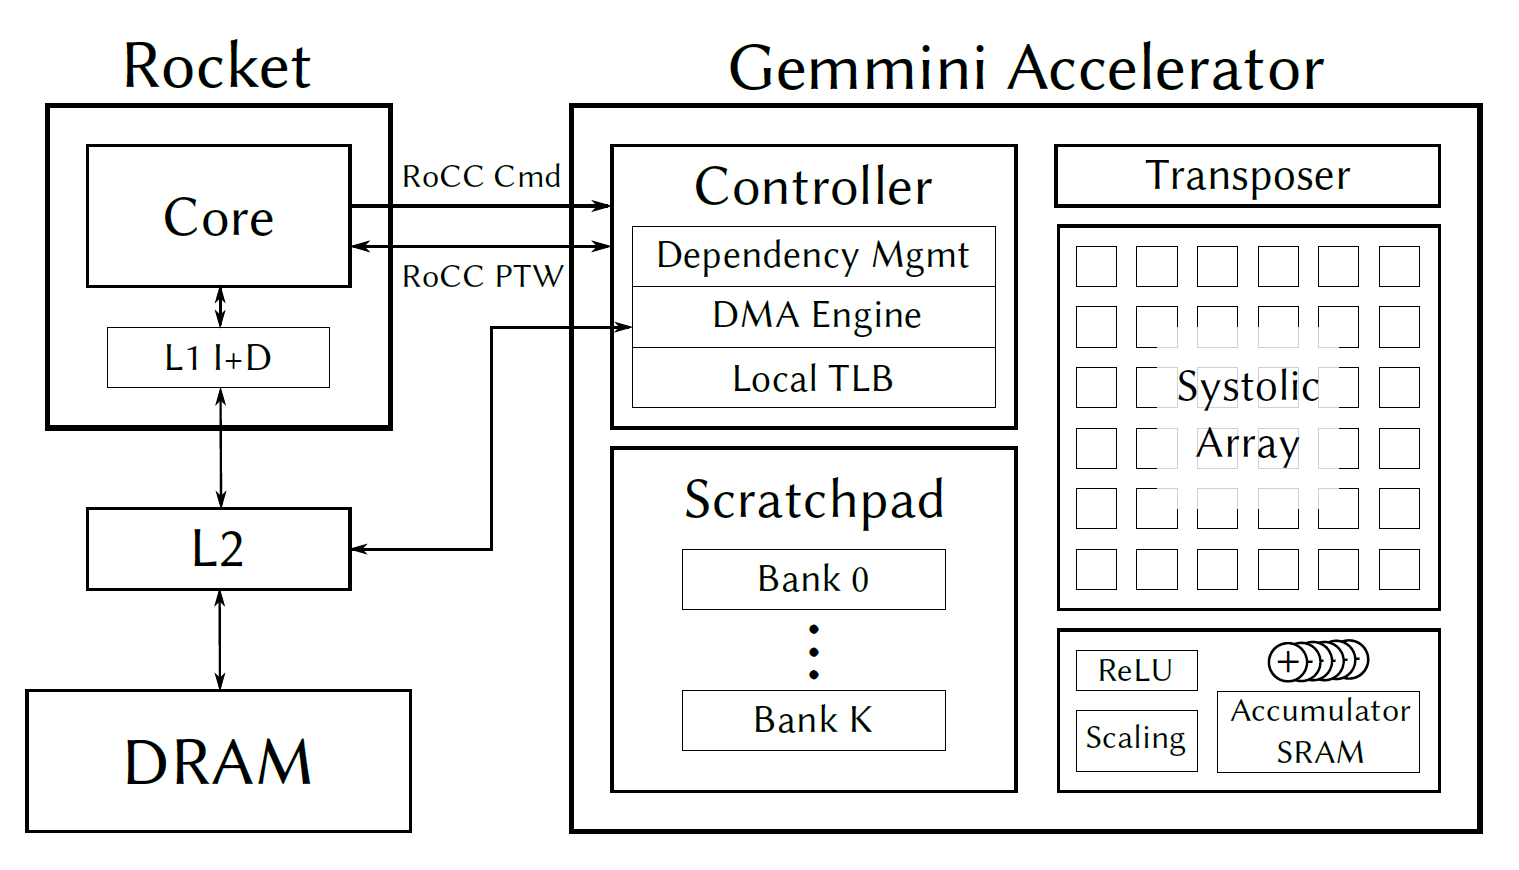
\includegraphics[scale=0.55]{./gemmini-system.png}
  \caption{Gemmini Accelerator Logic Design \parencite{gemminiGithub}}
  \label{fig:Gemmini_Accelerator}
\end{figure}

Gemmini is intended for integration with other \nameref{sec:Rocket_Chip}s, but can be configured to work with \nameref{sec:BOOM_Generator} chips as well.

\subsection{Hwacha}\label{sec:Hwacha}
\nocite{hwachaGithub}
\nocite{hwachaPresentation}
Like the \nameref{sec:Gemmini_Generator}, Hwacha is meant to be an accelerator.
Hwacha is a co-processor, designed to be run with other CPU processors, namely the \nameref{sec:Rocket_Chip}s.
Hwacha, like \nameref{sec:Gemmini_Generator}, is another SIMD co-processor, but designed to work with vectors instead or matrices.

It uses several alternative concepts in its design, including:
\begin{itemize}
\item A configurable register file, which is defined by software
\item A runtime-variable vector length register
\item Aggressive prefetching of memory, due to constant-stride memory accesses
\item Resolving memory references as early as possible.
\item Along with several others
\end{itemize}

These all feed into Hwacha's goal of maximizing the efficiency of an in-order vector microarchitecture.
It was designed to be usable with another CPU to run an operating system that supports unified virtual memory and restartable exceptions.
A block-level diagram of the major components in the Hwacha coprocessor is shown in \Cref{fig:Hwacha_Accelerator}

\begin{figure}[h!tbp]
  \centering
  % TODO: Recreate as vector image?
  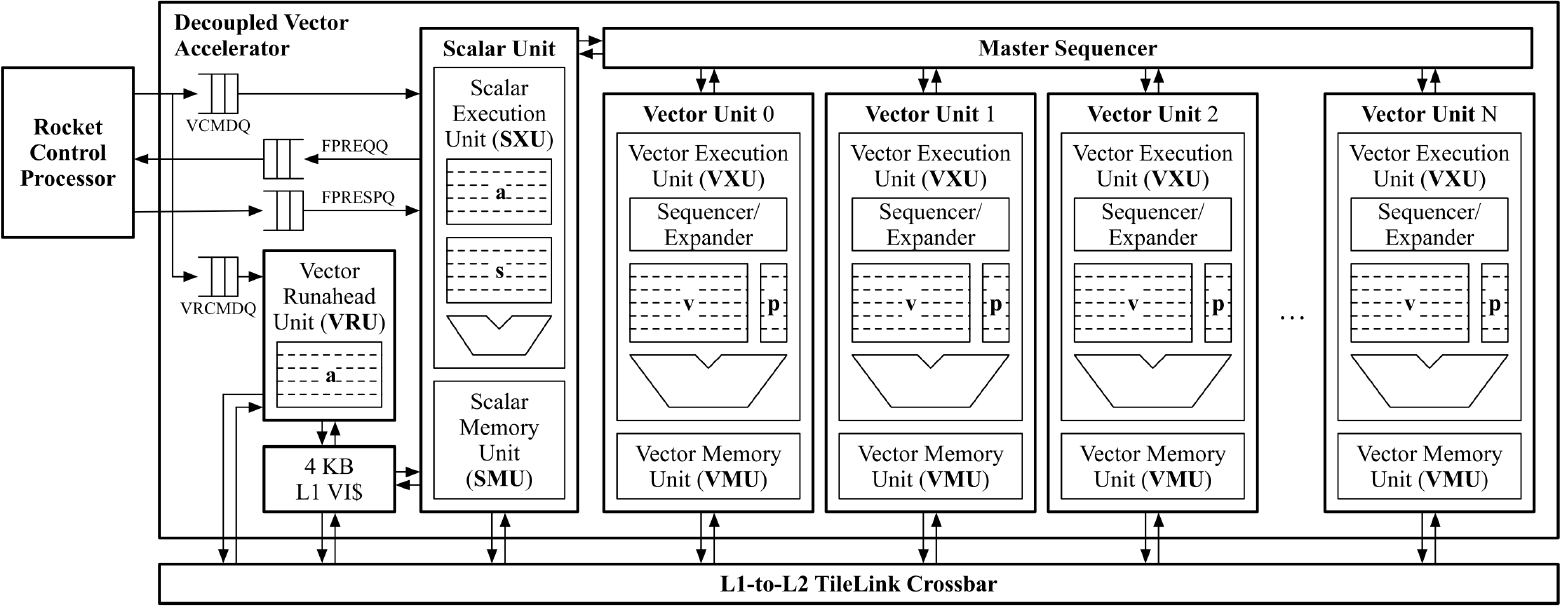
\includegraphics[scale=0.42]{./hwacha-system.png}
  \caption{Hwacha Design~\cite[p.~11]{hwachaPresentation}}
  \label{fig:Hwacha_Accelerator}
\end{figure}

\subsection{Icenet}\label{sec:Icenet_Generator}
\nocite{icenetGithub}
Icenet is a generator that is no less interesting, but less applicable to our uses.
It is intended to provide Ethernet-based networking components in support of the \nameref{sec:FireSim_Simulator} design simulator.
Like all other components in Chipyard, this is also parameterizable, allowing for multiple \Glspl{nic} to be defined.

\subsection{NVDLA}\label{sec:NVDLA_Generator}
\subsection{RISC-V Sodor}\label{sec:RISC-V_Sodor}
\subsection{Rocket-Chip}\label{sec:Rocket_Chip}
\subsection{SHA3}\label{sec:SHA3_Accelerators_Generator}
\subsection{SiFive Blocks}\label{sec:SiFive_Blocks}
\subsection{SiFive Cache}\label{sec:SiFive_Cache}
\subsection{\file{testchipip}}\label{sec:testchipip}

\section{Custom Configurations}\label{sec:Custom_Configurations}
Custom Configs can be created in the directory \mintinline{bash}{chipyard/generators/chipyard/src/main/scala/config/}.
For example, I created a new scala file called \file{NewTestConfig.scala} in the directory, allowing me to create a simulator from a class inside the NewTestConfig.scala file.
Example Configs can be found in  \file{RocketConfigs.scala} in the same directory.

% TODO: Include custom config example

\section{Verilator Simulator}\label{sec:Verilator_Simulator}

\subsection{FPGA Implementation}\label{sec:FPGA_Implementation}


\subsection{About}\label{sec:About}

\begin{figure}[h!tbp]
  \centering
  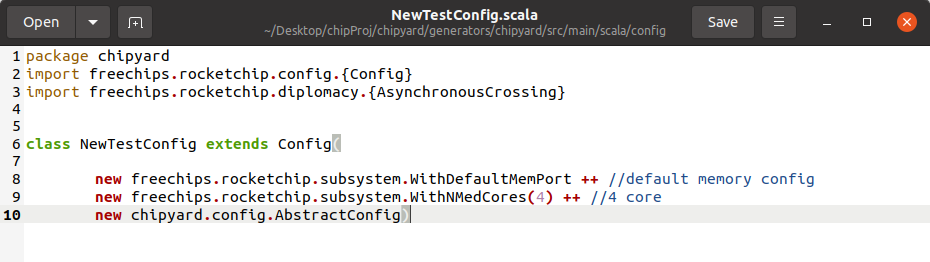
\includegraphics[width=0.7\linewidth]{./NewTestConfig.png}
  \caption{\file{NewTestConfig.scala}}
  \label{fig:newtestconfig}
\end{figure}

%%% Local Variables:
%%% mode: latex
%%% TeX-master: "../doc"
%%% End:


\backmatter{}
\printbibliography[heading=bibintoc]{}

\printacronyms{}
\printglossary{}
\end{document}